% !TEX program = xelatex
\documentclass[UTF8,a4paper,11pt,fontset=fandol]{ctexart}
\usepackage[margin=24mm,headheight=15pt]{geometry}
\usepackage{amsmath,amssymb,bm,booktabs,longtable,array,tabularx}
\usepackage{xcolor,fancyhdr,enumitem,needspace,tikz}
\usepackage[unicode,colorlinks=true,linkcolor=blue!45!black,urlcolor=blue!45!black]{hyperref}
\usepackage{xurl}
\definecolor{ink}{RGB}{30,54,78}
\ctexset{section={format=\Large\bfseries\color{ink}},subsection={format=\large\bfseries\color{ink}}}
\setlength{\parindent}{2em}
\setlength{\parskip}{3pt}
\setlength{\emergencystretch}{3em}
\setlist{nosep,leftmargin=2em}
\renewcommand{\arraystretch}{1.25}
\pagestyle{fancy}\fancyhf{}
\fancyhead[L]{\small QUANTUM 流体模块数值方法}
\fancyhead[R]{\small 源码审读 / 2026-09-13}
\fancyfoot[C]{\thepage}
\newcommand{\code}[1]{\nolinkurl{#1}}
\newcommand{\src}[1]{\textcolor{ink}{\small〔源码索引 #1〕}}
\newcommand{\thesis}[1]{\textcolor{ink}{\small〔论文：#1〕}}
\newcommand{\UU}{\bm{U}}
\newcommand{\vel}{\bm{u}}
\newcommand{\dd}{\,\mathrm{d}}
\newcommand{\dt}{\Delta t}
\newcommand{\mat}[1]{\mathsf{#1}}
\begin{document}
\begin{titlepage}
\vspace*{18mm}
{\color{ink}\Huge\bfseries QUANTUM 流体模块\par}
\vspace{6mm}
{\LARGE 数学模型与 CFD 数值方法\par}
\vspace{5mm}
{\large 数值格式细化修订版：参照范益朋博士论文\par}
\vspace{12mm}
\noindent\rule{\textwidth}{0.7pt}
\vspace{5mm}
\noindent\begin{tabularx}{\textwidth}{@{}lX@{}}
审读对象 & \path{D:/Chen/QUANTUM} 下的现行源码\\
主要范围 & \code{Modules/Hydrodynamics}，以及直接参与流体步的 Core 几何、速度重构与 App 接线\\
文档日期 & 2026 年 9 月 13 日\\
产物 & 本 LaTeX 源文件、修订版 PDF、源码定位与 SHA-256 清单\\
证据边界 & 源码审读和现有验证记录；本次不修改数值实现，不新增物理计算或宣称重新完成精度验收\\
\end{tabularx}
\vspace{9mm}
\noindent\textbf{核心判断}\par
本模块以不可压缩、变密度/变黏度牛顿流体为模型，在二维笛卡尔或无旋流轴对称网格上，采用压力居中、速度交错的有限体积离散。动量对流为空间一阶迎风、时间 AB2 显式组合；完整黏性应力采用 Crank--Nicolson 半隐式处理。现行检查式接口采用增量压力投影；均匀完整域和贴合流体域还通过速度--压力鞍点系统修正完整离散动量与连续性。

界面不是一套统一的 VOF 算法。普通 Hydro 使用水平集与平滑物性；运动喷嘴使用活动 Hermite 标量、与原生面通量兼容的速度重构、特征线输运和逐单元体积收支修正。固定粗细网格的若干部件已实现，但不等于运动喷嘴 AMR 全链已开放。
\vfill
\noindent\small 本文的数学式是对代码的整理；当经典算法名称不能完整概括当前实现时，给出实际矩阵、时间层和适用路径。源码定位见附录，阶段报告不作为比源码更高优先级的功能清单。
\end{titlepage}
\begingroup\small\setlength{\parskip}{0pt}\tableofcontents\endgroup
\newpage

\section{符号约定与论文参照}
本次修订参照范益朋博士论文《离子液体电喷雾推力器离子引出过程的多阶段耦合数值模拟》（大连理工大学，2026）：主要符号表（印刷页 XXI--XXII，PDF 第 27--28 页）及第 2 章，特别是式 (2.15)--(2.30)、图 2.1 与式 (2.31)--(2.36)。本文采用其“控制体、通量算子、黏性算子、矩阵系数”的展开方式；公式编号均为本报告自己的编号。\thesis{符号表；第 2.1 节}

\subsection{物理符号与代码名称的对应}
\begin{longtable}{@{}p{.15\textwidth}p{.35\textwidth}p{.43\textwidth}@{}}
\toprule 符号 & 含义 & 与论文/代码的关系\\\midrule\endhead
$\vel=(u,v)$ & 平面速度；RZ 写 $(u_r,u_z)$ & \code{ux,uy}；离散整列速度写 $\UU$\\
$p$，$\psi$ & 物理压强、压力修正量 & \code{p}、\code{pressurePotential_}；$\psi$ 不是电势或水平集\\
$\varphi$ & 水平集/相界面标量 & 与论文一致，替换前版水平集的 $\phi$；$\varphi<0$ 为液侧\\
$\phi$ & 电势 & 与论文一致；仅用于电学背景说明\\
$\rho,\mu$ & 密度、动力黏度 & \code{rho,mu}；在代码离散式中使用实际已归一化的黏度\\
$\gamma$，$\sigma$ & 表面张力、电导率 & 与论文一致；表面张力不再用 $\sigma$ 表示\\
$\bm D$ & 应变率张量 & $\bm D=(\nabla\vel+\nabla\vel^T)/2$；$\bm\tau=2\mu\bm D$\\
$\mathcal L_p,\mathcal L_u,\mathcal L_v$ & 压力原控制体与两速度对偶控制体 & $\Delta V$ 为相应体积；平面单位厚度时为面积 $\Delta A$\\
$S_e,S_w,S_n,S_s$ & 各控制体四侧的几何面测度 & 平面为边长；RZ 为回转面积；$e/w/n/s$ 指东/西/北/南\\
$q_\ell$，$\dot m_\ell$ & 质量通量密度、积分质量流率 & $q_\ell=\rho_\ell u_{n,\ell}$，$\dot m_\ell=q_\ell S_\ell$；代码旧 \code{_qEast} 通常已含 $S_e$\\
$Q_f$，$Q_f^-$ & 原生面体积流率、液相部分体积流率 & 不含密度；必须与 $q,\dot m$ 区分\\
$\mathcal C_u,\mathcal V_u$ & 对流积分算子、完整黏性应力积分算子 & $\mathcal V_u$ 含完整 $2\mu\bm D$，CN 系数另显式写 $1/2$\\
$G_h,\mathcal D_h$ & 面梯度、除单元体积的离散散度 & $\mat B$ 为未除体积的通量矩阵，$\mat C$ 为积分压力梯度；不与 $\bm D$ 混用\\
$\mat A,\mat M$ & 动量矩阵、面质量对角阵 & $\mat M_{ff}=\rho_f\Delta V_f$；$\mat C$ 与对流 $\mathcal C_u$ 字体/下标不同\\
\bottomrule
\end{longtable}
在后续数学式中，\code{surfaceTension} 的数值对应 $\gamma$，历史配置/日志中的 \code{sigma} 字符串保持原名。代码标量物性和力均按实际调用单位解释；以有量纲方程作推导后，使用已归一化系数时省去波浪号。

\subsection{空间索引与时间层定义}
统一以压力单元中心 $(i,j)$ 为全局索引：
\begin{equation}
 p_{i,j},\rho_{i,j},\mu_{i,j};\qquad
 u_{i+1/2,j};\qquad v_{i,j+1/2};\qquad
 \varphi_{i+1/2,j+1/2}.
\end{equation}
论文图 2.1(b) 将 $u$ 控制体中心局部重标为 $(i,j)$；本文保持上述全局索引，并用 $P,E,W,N,S$ 表示当前动量行的同分量邻点，避免在压力式和速度式中无提示切换原点。

\begin{longtable}{@{}p{.18\textwidth}p{.75\textwidth}@{}}
\toprule 上标 & 精确定义\\\midrule\endhead
$n,n-1,n+1$ & 已接受旧速度、再前一层速度、接受的新速度；\code{uxPre/uyPre} 在步前存 $n-1$，NS 求解后改存 $n$\\
$\star$ & 黏性隐式动量预测速度，尚未投影；对应 \code{uxMid/uyMid}，不是时间 $n+1/2$ 的已接受速度\\
$P$ & 本报告专用：初次压力投影之后、完整耦合修正之前\\
$[n]$ & 本次装配冻结的物性/力系数。生产路径按其旧界面提供，不表示已经求得真实半时层\\
$n+1/2$ & 只在论文格式对照或已明确构造的时间平均中使用；不把代码的 $\rho^{[n]},\mu^{[n]},\bm f^{[n]}$ 直接改标签\\
$(k)$ & 同一个物理时间步内部的非线性体积修正迭代；不是新物理时间\\
\bottomrule
\end{longtable}

\subsection{论文写法与当前代码的四处关键差别}
\begin{enumerate}
\item 论文式 (2.16)--(2.18) 为不含历史压强的非增量投影。现行检查式接口在预测右端加入 $-G_hp^n$，求 $\psi$ 后累积压强，并在适用路径再解完整耦合修正；保留的旧重载才具有论文式的非增量语义。
\item 论文式 (2.21) 列出变步长权重；当相邻步长相等时为 $\alpha=3/2,\beta=-1/2$。当前 NS 装配直接使用 $-1.5\mathcal C^n+0.5\mathcal C^{n-1}$，检查式接口锁定固定步长；不据论文认定代码已有变步长 NS。
\item 论文式 (2.2) 定义 $\bm D$ 含 $1/2$，式 (2.16)、(2.22) 的单侧 CN 黏性项为 $\nabla\cdot(\mu\bm D)$；而式 (2.25)--(2.27) 又展开为完整应力 $\mu(\nabla\vel+\nabla\vel^T)$。按所印公式直接连用存在因子 2 的不一致。本文统一定义完整应力算子 $\mathcal V$，并写成 $-\mathcal V^\star/2$ 和 $+\mathcal V^n/2$，与代码矩阵的 $0.5$ 系数核对。
\item 论文式 (2.28)--(2.30) 的 $q$ 尚未乘侧面测度；代码的 \code{_qWest/_qEast} 已乘边长或回转面积。本文用 $q$ 与 $\dot m=qS$ 分开，防止在对流项重复乘几何因子。
\end{enumerate}
以上是符号和离散对应关系，不改写论文原件，也不将论文中的算法描述当作当前代码的功能声明。\src{S02,S07,S09}\thesis{式 (2.2)、(2.16)--(2.30)}


\section{范围、入口与方法总览}
\subsection{三类流体入口必须分开理解}
\begin{longtable}{@{}p{.18\textwidth}p{.37\textwidth}p{.38\textwidth}@{}}
\toprule 路径 & 实际调用与状态 & 数值含义及范围\\\midrule\endhead
独立 Hydro / Hydro 驱动的 EHD & \code{HydrodynamicsModule::runCoupled} 调用 \code{solve/solveRZ}，传入 \code{HydroSolveOptions} & 固定步长，增量压力。标准字典入口要求完整均匀网格；底层封闭域另有固定 2:1 叶网格投影。\\
贴合流体域 / 喷嘴 & \code{ElectrosprayTimeLoop} 调用 \code{solveFittedRZ}，传入 \code{HydroFittedDomain} & 只以活动流体单元和自由速度面为未知量；固体法向约束被消元。压力库和压力出口具有半对偶控制体。\\
旧几何耦合接口 & 带 \code{SharpInterface}、\code{ImmersedGeometry} 的 \code{solve/solveRZ} 重载 & 保留非增量压力、IBM 表面力/蒸发/直接力修正；不是现行喷嘴贴合域步的同义接口。\\
\bottomrule
\end{longtable}
同一 Hydro 对象不能在接受时间步后混用不同压力语义，贴合域历史也不能切到完整域。普通接口失败可能已经改变速度、压力或历史场，不能原地改小步长后直接重试；喷嘴 App 的后续界面/电学失败同样要求终止该次运行。\src{S01,S02,S09,S20}

\subsection{按 CFD 环节归纳}
\begin{longtable}{@{}p{.20\textwidth}p{.73\textwidth}@{}}
\toprule 环节 & 现行方法\\\midrule\endhead
控制方程 & 不可压缩 NS；牛顿黏性应力；外加体积力及界面力。RZ 不包含旋流速度方程。\\
空间布局 & 单元中心 $p,\rho,\mu$；竖直面 $u_x/u_r$，水平面 $u_y/u_z$；顶点水平集及部分物性/导数。\\
动量对流 & 对偶控制体质量通量乘供体速度，一阶迎风；不是 MUSCL、QUICK 或 WENO 动量通量。\\
黏性 & 法向应力含系数 $2\mu$，剪切应力包含两速度交叉导数；中心型离散和 CN 时间组合。\\
压力耦合 & 预测速度、变系数压力增量投影；支持路径再加完整动量--连续性联立修正。\\
界面运动 & 两时间层速度的中点回溯；普通接口用父单元双二次/根单元双线性插值，喷嘴用活动双三次 Hermite 标量。\\
界面力 & 与压力梯度相容的交错面毛细力；可选历史轮廓或共享 Hermite 几何。附加牵引/电力从单元或面端口进入。\\
守恒修正 & 喷嘴按逐单元液相体积与梯形时间积分相通量修正 Hermite 自由度；并非独立推进 VOF 体积分数。\\
线性代数 & SuperLU 稀疏直接解；动量、压力、耦合分别检查残差，矩阵完全相同时复用分解。\\
\bottomrule
\end{longtable}

\section{数学模型、相定义和单位}
\subsection{不可压缩两相牛顿流体}
设 $\varphi<0$ 为负相（喷嘴中为液相），$\varphi>0$ 为正相，$\bm n=\nabla\varphi/|\nabla\varphi|$ 从负相指向正相。每一相内可将模型写为
\begin{align}
 \nabla\cdot\vel &=0,\label{eq:mass}\\
 \rho\left(\partial_t\vel+\vel\cdot\nabla\vel\right)
 &=-\nabla p+\nabla\cdot\bm\tau+\rho\bm a+\bm f_\Gamma+\bm f_{\rm ext},\label{eq:ns}\\
 \bm\tau&=2\mu\bm D=\mu\left(\nabla\vel+\nabla\vel^T\right),\\
 \partial_t\varphi+\vel\cdot\nabla\varphi&=0.\label{eq:ls}
\end{align}
论文式 (2.1) 的守恒动量写法为
\begin{equation}
 \partial_t(\rho\vel)+\nabla\cdot(\rho\vel\otimes\vel)
 =-\nabla p+\nabla\cdot(2\mu\bm D)+\rho\bm a+\bm f_\Gamma+\bm f_{\rm ext}.
\end{equation}
当 $\partial_t\rho+\nabla\cdot(\rho\vel)=0$ 成立时，它与式~\eqref{eq:ns} 等价。两相密度不同而各相不可压缩时，$\nabla\cdot\vel=0$ 并不允许把 $\rho$ 从动量通量中任意提出。\thesis{式 (2.1)--(2.2)}

这是一种单流场描述：两相共享压力与速度自由度，通过不同物性和界面载荷耦合。当前流体步没有能量方程、状态方程、声波求解或湍流闭合。旧蒸发速度端口的存在，不能解释为现行 Hydro 已联立求解完整热质传递模型。

\textbf{连续模型与离散守恒需要区分。}式~\eqref{eq:ns} 是相内模型；实际动量代码使用质量通量形式的迎风对流，但时间质量系数由当前调用给出的 $\rho$ 冻结。代码并未在同一 NS 步内联立推进一条与动量通量严格一致的离散密度方程。因此，不能仅凭“有限体积”称其已证明两相质量--动量一致守恒或离散动能守恒。\src{S01,S02,S07,S21}

\subsection{普通 Hydro 与喷嘴的物性离散不同}
普通 \code{twoPhase} 路径先在顶点计算
\begin{align}
 H_\epsilon(\varphi)&=\tfrac12\left[1+\tanh\left(\frac{\varphi}{2\epsilon}\right)\right],\\
 \rho_v&=\rho_-(1-H_\epsilon)+\rho_+H_\epsilon,\qquad
 \mu_v=\mu_-(1-H_\epsilon)+\mu_+H_\epsilon,
\end{align}
再用已有顶点到单元场转换得到 $\rho_K,\mu_K$。这里 $\epsilon$ 是代码 \code{thickness} 的准确位置，不能漏掉分母中的 $2$。旧无显式材料参数重载还将黏度乘以全局 $Re^{-1}$；现行独立配置不能无条件套用这一旧归一化。\src{S02,S12}

喷嘴 \code{updateElectrosprayHydroMaterials} 则按活动单元的液/气相 ID 赋纯相常物性；运动后通过当前 Hermite 标量在单元中心的符号更新相 ID。顶点物性是相邻活动单元物性的算术平均，不读取固体物性。它没有把逐单元几何液体体积直接当作混合密度权重。由此，\textbf{材料场、受力层指标和守恒所用几何体积是三个不同对象}。\src{S21}

\subsection{RZ 方程与几何测度}
以 $x=r,y=z$，速度为 $(u_r,u_z)$，无 $u_\theta$。连续性为
\begin{equation}
 \frac{1}{r}\frac{\partial (r u_r)}{\partial r}+\frac{\partial u_z}{\partial z}=0.
\end{equation}
主要应力为
\begin{equation}
 \tau_{rr}=2\mu\partial_r u_r,\quad
 \tau_{zz}=2\mu\partial_z u_z,\quad
 \tau_{rz}=\mu(\partial_z u_r+\partial_r u_z),\quad
 \tau_{\theta\theta}=2\mu u_r/r.
\end{equation}
径向与轴向黏性项分别是
\begin{align}
 (\nabla\cdot\bm\tau)_r
 &=r^{-1}\partial_r(r\tau_{rr})+\partial_z\tau_{rz}-\tau_{\theta\theta}/r,\\
 (\nabla\cdot\bm\tau)_z
 &=r^{-1}\partial_r(r\tau_{rz})+\partial_z\tau_{zz}.
\end{align}
控制体积为 $V_K=\pi(r_e^2-r_w^2)\Delta z$；径向面面积为 $2\pi r_f\Delta z$，轴向面面积为 $\pi(r_e^2-r_w^2)$。二维平面路径按单位面外厚度计面积/体积。原生同层矩形网格可写成 $V_K=2\pi r_K\Delta r\Delta z$，但贴合域保留真实中心与端点求测度，不能将所有半对偶体积都替换成“完整体积的一半”。

现行 RZ 路径显式加入环向应力项 $-2\mu u_r/r^2$ 的 CN 贡献：内部行向矩阵加入 $\mu V_f/r_f^2$，右端减去同系数乘旧 $u_r$。压力边界的半对偶体积使用含 \code{log1p} 的积分权重。轴线上 $u_r=0$、$u_z$ 关于 $r$ 为偶函数；轴面面积为零，不对轴上的 $1/r$ 作任意截断。\src{S05,S07,S08,S10}

\subsection{代码单位与 SI}
独立 Hydro 的配置是代码单位。喷嘴由 App 显式构造
\begin{equation}
 U_0=L_0/T_0,\qquad P_0=\rho_0U_0^2,\qquad
 \mu_0=\rho_0U_0L_0,
\end{equation}
若另用参考动力黏度 $\mu_c$ 定义 $Re=\rho_0U_0L_0/\mu_c$，则当前装配消费的黏度是
\begin{equation}
 \mu_{\rm code}=\frac{\mu_{\rm SI}}{\rho_0U_0L_0}
 =\frac{\widetilde\mu}{Re},\quad
 \gamma_{\rm code}=\frac{\gamma_{\rm SI}}{\rho_0U_0^2L_0}=\frac1{We},\quad
 \widetilde\mu=\mu_{\rm SI}/\mu_c.
\end{equation}
因此本文离散黏性式中的 $\mu$ 已包含所需的 $Re^{-1}$，不能再额外乘一遍。这里 $We$ 按当前表面张力定义；$L_0,U_0,\rho_0$ 对应论文的特征长度、速度、密度。
其中 $\rho_0$ 取配置液体密度；体积力尺度为 $P_0/L_0$。RZ 通量已经包含回转面积，不能再乘一次 $2\pi r$。文中矩阵均使用调用方一致的代码单位，最终物理输出是否为 SI 应以 App 的输出标签为准。\src{S21}

\section{交错控制体上的空间离散格式}
\subsection{压力单元与两个动量模板}
图~\ref{fig:staggered} 给出本报告统一索引的几何含义。竖直面上的 $u$ 横向控制体宽度为两侧压力中心间距；其南北边经过原生顶点。$v$ 控制体以同样方式转置。
\begin{figure}[htbp]\centering
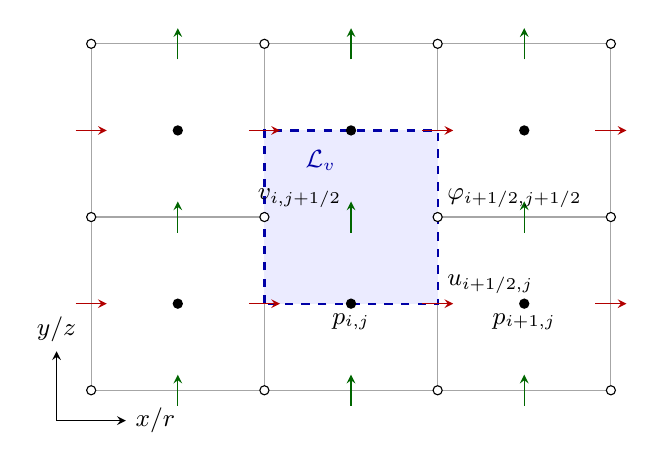
\begin{tikzpicture}[scale=1.1,>=stealth,font=\small]
\draw[gray!70,step=2] (0,0) grid (6,4);
\fill[blue!8] (2,1) rectangle (4,3);
\draw[blue!65!black,dashed,thick] (2,1) rectangle (4,3);
\foreach \x in {1,3,5}\foreach \y in {1,3}\fill (\x,\y) circle (1.7pt);
\foreach \x in {0,2,4,6}\foreach \y in {1,3}\draw[->,red!70!black] (\x-.18,\y)--(\x+.18,\y);
\foreach \x in {1,3,5}\foreach \y in {0,2,4}\draw[->,green!40!black] (\x,\y-.18)--(\x,\y+.18);
\foreach \x in {0,2,4,6}\foreach \y in {0,2,4}\draw[fill=white] (\x,\y) circle (1.5pt);
\node[below] at (3,1){$p_{i,j}$};\node[below] at (5,1){$p_{i+1,j}$};
\node[above right] at (4,1){$u_{i+1/2,j}$};
\node[above left] at (3,2){$v_{i,j+1/2}$};
\node[above right] at (4,2){$\varphi_{i+1/2,j+1/2}$};
\node[blue!65!black] at (2.65,2.65){$\mathcal L_v$};
\draw[->] (-.4,-.35)--(.4,-.35) node[right]{$x/r$};
\draw[->] (-.4,-.35)--(-.4,.45) node[above]{$y/z$};
\end{tikzpicture}
\caption{原生压力、面速度和顶点水平集的布局；阴影示例为 $v_{i,j+1/2}$ 的对偶控制体。根据源码关系重新绘制，参照论文图 2.1 的表示方式。}
\label{fig:staggered}
\end{figure}
为缩短完整模板，分别对每个动量行定义下列局部名字；下标 $NE,NW,SE,SW$ 专指另一速度分量在交错角点的位置。
\begin{center}\small
\begin{tabular}{@{}lll@{}}\toprule
位置 & $u$ 行模板 & $v$ 行模板\\\midrule
$P$ & $u_{i+1/2,j}$ & $v_{i,j+1/2}$\\
$E,W$ & $u_{i+3/2,j},u_{i-1/2,j}$ & $v_{i+1,j+1/2},v_{i-1,j+1/2}$\\
$N,S$ & $u_{i+1/2,j+1},u_{i+1/2,j-1}$ & $v_{i,j+3/2},v_{i,j-1/2}$\\
$NE,NW$ & $v_{i+1,j+1/2},v_{i,j+1/2}$ & $u_{i+1/2,j+1},u_{i-1/2,j+1}$\\
$SE,SW$ & $v_{i+1,j-1/2},v_{i,j-1/2}$ & $u_{i+1/2,j},u_{i-1/2,j}$\\\bottomrule
\end{tabular}
\end{center}
以下显式模板用于完整同层、均匀矩形内部行。边界缺失邻点与粗细面需按后文专门规则装配，不将上述邻点表用于读取固体或不存在的自由度。

\subsection{物性与体积力的采样位置}
对 $u$ 行，本步材料取值为
\begin{align}
 \rho_P&=\tfrac12(\rho_{i,j}+\rho_{i+1,j}),&
 \rho_e&=\rho_{i+1,j},&\rho_w&=\rho_{i,j},\\
 \rho_n&=\rho^{\rm vert}_{i+1/2,j+1/2},&
 \rho_s&=\rho^{\rm vert}_{i+1/2,j-1/2}.\label{eq:material-template}
\end{align}
$\mu_e,\mu_w,\mu_n,\mu_s$ 取对应位置的黏度；$v$ 行交换 $x/y$：南北取单元物性，东西取顶点物性，质量用上下单元密度平均。这里的顶点值来自实际材料更新路径，而不是在这一步另做谐均。

单元体积力 $f_x$ 对完整 $u$ 行的载荷是 $\Delta V_u(f_{x,i,j}+f_{x,i+1,j})/2$，$v$ 行同理。若通过面力端口给出 $f_{x,P}^{\rm face}$，直接增加 $\Delta V_u f_{x,P}^{\rm face}$。这些 $f$ 都是力密度而非加速度；重力/给定加速度先构成 $\rho\bm a$。\src{S02,S07,S08}

\subsection{四个方向的对流通量与供体值}
对 $u$ 行，令时间上标 $m=n$ 或 $n-1$，几何与物性均固定为本步输入：
\begin{align}
 q_e^m&=\rho_e\tfrac12(u_P^m+u_E^m),&q_w^m&=\rho_w\tfrac12(u_P^m+u_W^m),\\
 q_n^m&=\rho_n\tfrac12(v_{NE}^m+v_{NW}^m),&q_s^m&=\rho_s\tfrac12(v_{SE}^m+v_{SW}^m).
\end{align}
每个 $q$ 的正方向均为正坐标方向，并非控制体向外方向。四个供体值为
\begin{align}
 u_e^{{\rm up},m}&=\begin{cases}u_P^m,&q_e^m>0,\\u_E^m,&q_e^m\le0,\end{cases}&
 u_w^{{\rm up},m}&=\begin{cases}u_W^m,&q_w^m>0,\\u_P^m,&q_w^m\le0,\end{cases}\\
 u_n^{{\rm up},m}&=\begin{cases}u_P^m,&q_n^m>0,\\u_N^m,&q_n^m\le0,\end{cases}&
 u_s^{{\rm up},m}&=\begin{cases}u_S^m,&q_s^m>0,\\u_P^m,&q_s^m\le0.\end{cases}
\end{align}
最终对流积分算子是
\begin{equation}
 \mathcal C_u^m=\underbrace{q_e^m S_e}_{\dot m_e^m}u_e^{{\rm up},m}
 -q_w^m S_wu_w^{{\rm up},m}+q_n^m S_nu_n^{{\rm up},m}-q_s^m S_su_s^{{\rm up},m}.
 \label{eq:explicit-convection}
\end{equation}
对 $v$ 行，同分量平均移到南北侧：
\begin{align}
 q_n^m&=\rho_n(v_P^m+v_N^m)/2,&q_s^m&=\rho_s(v_P^m+v_S^m)/2,\\
 q_e^m&=\rho_e(u_{NE}^m+u_{SE}^m)/2,&q_w^m&=\rho_w(u_{NW}^m+u_{SW}^m)/2.
\end{align}
按相同供体规则将 $u$ 换成 $v$ 得到 $\mathcal C_v^m$。零通量时供体选哪一侧不改变乘积。\textbf{平均的是输运速度，迎风的是被输运分量}：空间格式是一阶供体法，没有斜率限制器、高阶上风重构或动量 WENO。\src{S02,S07}\thesis{式 (2.28)--(2.30)}

\subsection{完整黏性算子的两个分量}
以 $h_x=\Delta x,h_y=\Delta y$，$u$ 行的应力积分为
\begin{align}
 \mathcal V_u(u,v)={}&2\mu_e\frac{u_E-u_P}{h_x}S_e
                  -2\mu_w\frac{u_P-u_W}{h_x}S_w\notag\\
 &+\mu_n\left(\frac{u_N-u_P}{h_y}+\frac{v_{NE}-v_{NW}}{h_x}\right)S_n\notag\\
 &-\mu_s\left(\frac{u_P-u_S}{h_y}+\frac{v_{SE}-v_{SW}}{h_x}\right)S_s.
 \label{eq:visc-u}
\end{align}
$v$ 行为
\begin{align}
 \mathcal V_v(u,v)={}&\mu_e\left(\frac{v_E-v_P}{h_x}+\frac{u_{NE}-u_{SE}}{h_y}\right)S_e\notag\\
 &-\mu_w\left(\frac{v_P-v_W}{h_x}+\frac{u_{NW}-u_{SW}}{h_y}\right)S_w\notag\\
 &+2\mu_n\frac{v_N-v_P}{h_y}S_n-2\mu_s\frac{v_P-v_S}{h_y}S_s.
 \label{eq:visc-v}
\end{align}
平面内部 $S_e=S_w=h_y,S_n=S_s=h_x$。式~\eqref{eq:visc-u}--\eqref{eq:visc-v} 中的 $2\mu$ 是完整法向应力，剪切包含交叉导数；CN 的 $1/2$ 尚未放入这两个算子。变黏度时不能用两个独立的 $\mu\nabla^2$ 标量式替代。\src{S02,S07}

\subsection{一条动量矩阵行的全部非零系数}
对 $u$ 行，把 $\rho_P\Delta V_u u_P^\star/\dt-\mathcal V_u(u^\star,v^\star)/2$ 展开：
\begin{equation}
 a_Pu_P^\star+a_Eu_E^\star+a_Wu_W^\star+a_Nu_N^\star+a_Su_S^\star
 +\sum_{c\in\{NE,NW,SE,SW\}}b_cv_c^\star=b_{u,P}.
\end{equation}
同层平面或 RZ 的非环向部分系数如下：
\begin{align}
 a_P&=\frac{\rho_P\Delta V_u}{\dt}
       +\frac{\mu_eS_e+\mu_wS_w}{h_x}
       +\frac{\mu_nS_n+\mu_sS_s}{2h_y},\label{eq:u-diag}\\
 a_E&=-\frac{\mu_eS_e}{h_x},\quad a_W=-\frac{\mu_wS_w}{h_x},\quad
 a_N=-\frac{\mu_nS_n}{2h_y},\quad a_S=-\frac{\mu_sS_s}{2h_y},\\
 b_{NE}&=-\frac{\mu_nS_n}{2h_x},\quad b_{NW}=+\frac{\mu_nS_n}{2h_x},\quad
 b_{SE}=+\frac{\mu_sS_s}{2h_x},\quad b_{SW}=-\frac{\mu_sS_s}{2h_x}.
\end{align}
对 $v$ 行写相同形式，但 $a$ 乘 $v$、$b$ 乘 $u$：
\begin{align}
 a_P&=\frac{\rho_P\Delta V_v}{\dt}
       +\frac{\mu_eS_e+\mu_wS_w}{2h_x}
       +\frac{\mu_nS_n+\mu_sS_s}{h_y},\\
 a_E&=-\frac{\mu_eS_e}{2h_x},\quad a_W=-\frac{\mu_wS_w}{2h_x},\quad
 a_N=-\frac{\mu_nS_n}{h_y},\quad a_S=-\frac{\mu_sS_s}{h_y},\\
 b_{NE}&=-\frac{\mu_eS_e}{2h_y},\quad b_{SE}=+\frac{\mu_eS_e}{2h_y},\quad
 b_{NW}=+\frac{\mu_wS_w}{2h_y},\quad b_{SW}=-\frac{\mu_wS_w}{2h_y}.
\end{align}
右端包括旧质量项、$-3\mathcal C^n/2+\mathcal C^{n-1}/2$、$\mathcal V^n/2$、体积力及历史压强，具体见下一节。上述系数逐项对应 \code{appendRadialMatrix/appendAxialMatrix} 及平面 \code{buildMomenMatrix} 的 triplet。\src{S02,S07}

\subsection{轴对称面测度与环向黏性离散}
令当前速度面半径为 $r_P$，完整同层对偶体尺寸为 $h_r,h_z$。两类行均使用
\begin{align}
 S_e&=2\pi(r_P+h_r/2)h_z,&S_w&=2\pi(r_P-h_r/2)h_z,\\
 S_n=S_s&=\pi[(r_P+h_r/2)^2-(r_P-h_r/2)^2]=2\pi r_Ph_r,\\
 \Delta V&=2\pi r_Ph_rh_z.
\end{align}
将这些实际面测度代入对流和黏性式。径向行还必须加上柱坐标应力散度的环向贡献
\begin{equation}
 \mathcal V_r^{\rm full}=\mathcal V_u-\frac{2\mu_P\Delta V}{r_P^2}u_{r,P}.
\end{equation}
因此在式~\eqref{eq:u-diag} 的对角上增加 $\zeta_P=\mu_P\Delta V/r_P^2$，右端旧黏性项相应减去 $\zeta_Pu_{r,P}^n$；轴向行无此项。$\mu_P$ 为该行两侧黏度平均，粗细行用相同虚拟子单元材料插值。轴面径向速度为约束，不套用 $r_P=0$ 的自由速度行公式。

这些化简式适用于规则矩形。实际贴合域在微小坐标下保留原端点/中心算术；原生剪切右端可能以真实中点差代替 $h$。边界径向半对偶体用环带积分，不能一律套 $\Delta V/2$。\src{S05,S07,S08,S10}

\subsection{粗细面梯度的明确插值形式}
对粗单元 $C$ 的虚拟子中心 $\bm x_s=\bm x_C+(\pm h_x/4,\pm h_y/4)$，实际选择粗中心及两个按方向优先序取得的邻中心组成三点支持。令局部坐标 $\xi_k=(x_k-x_C)/h_x,\eta_k=(y_k-y_C)/h_y$，则
\begin{equation}
 \mat X=\begin{bmatrix}1&\xi_1&\eta_1\\1&\xi_2&\eta_2\\1&\xi_3&\eta_3\end{bmatrix},\quad
 \bm w^T=\begin{bmatrix}1&\xi_s&\eta_s\end{bmatrix}
 (\mat X^T\mat X)^{-1}\mat X^T,
 \quad p_s=\sum_kw_kp_k.
\end{equation}
这是实际压力/密度共享的\emph{线性}基，不是论文式 (2.31) 的六列二次基。压力虚拟子单元路径调用三点默认分支；其它速度辅助插值按各自模板保留，不据一个通用最小二乘函数的选项推断所有场都采用同阶。

若粗侧在负坐标、细单元 $F$ 在正坐标，当前面梯度与密度为
\begin{equation}
 (G_hp)_f=\frac{p_F-\sum_kw_kp_k}{h_{\rm fine}},\qquad
 \rho_f=\frac{\rho_F+\sum_kw_k\rho_k}{2}.
\end{equation}
粗侧在另一边时相应换号。\code{visitGradient} 发出 $1/h_{\rm fine}$ 与 $-w_k/h_{\rm fine}$，同一实际子面的系数装入两侧连续性方程且符号相反。不能换成 $p_F-p_C$ 除真实粗细中心距，也不能只改细单元一侧。

当前此共享算子已提取到 \code{Solvers/Operators/QuadtreeFaceGradient.h}，\code{HydroNativePressureStencil} 保留兼容别名和面物性评价；算法仍为上述原插值。\src{S03,S04,S30}\thesis{式 (2.31)--(2.36)}


\section{时间离散、压力投影与完整耦合修正}
\subsection{按时间层写出的两个动量预测式}
取 $\alpha=3/2,\beta=-1/2$。在一个完整同层 $u$ 控制体中，本步实际预测式为
\begin{align}
 \frac{\rho_P^{[n]}\Delta V_u}{\dt}u_P^\star
 -\frac12\mathcal V_u^{[n]}(u^\star,v^\star)
 ={}&\frac{\rho_P^{[n]}\Delta V_u}{\dt}u_P^n
 -\big[\alpha\mathcal C_u^{[n]}(\UU^n)+\beta\mathcal C_u^{[n]}(\UU^{n-1})\big]\notag\\
 &+\frac12\mathcal V_u^{[n]}(u^n,v^n)
 +\Delta V_u f_{x,P}^{[n]}
 -\Delta V_u\frac{p^n_{i+1,j}-p^n_{i,j}}{h_x}.
 \label{eq:cn-ab-u}
\end{align}
$v$ 行对应为
\begin{align}
 \frac{\rho_P^{[n]}\Delta V_v}{\dt}v_P^\star
 -\frac12\mathcal V_v^{[n]}(u^\star,v^\star)
 ={}&\frac{\rho_P^{[n]}\Delta V_v}{\dt}v_P^n
 -\big[\alpha\mathcal C_v^{[n]}(\UU^n)+\beta\mathcal C_v^{[n]}(\UU^{n-1})\big]\notag\\
 &+\frac12\mathcal V_v^{[n]}(u^n,v^n)
 +\Delta V_v f_{y,P}^{[n]}
 -\Delta V_v\frac{p^n_{i,j+1}-p^n_{i,j}}{h_y}.
 \label{eq:cn-ab-v}
\end{align}
RZ 径向行使用前节的 $\mathcal V_r^{\rm full}$，$h_x,h_y$ 换为 $h_r,h_z$。这里 $[n]$ 提醒读者：两个对流历史都使用本次材料系数，而速度分别为 $n,n-1$。压力库、出口和约束行按下一节的实际边界补充。

式~\eqref{eq:cn-ab-u}--\eqref{eq:cn-ab-v} 是对流 AB2 显式、应力 CN 隐式--显式各半。代码没有把 $\rho^{[n]}u^{n+1}-\rho^{[n-1]}u^n$ 作为该时间质量项，也未在 NS 中额外保存一致密度通量方程。初始化常取 $\UU^{-1}=\UU^0$，首步对流组合退为 $-\mathcal C(\UU^0)$。

\subsection{矩阵形式与代码变量对应}
令 $\mat M_{ff}=\rho_f^{[n]}\Delta V_f$，$\mat L\UU$ 表示完整应力积分，则
\begin{align}
 \mat A&=\mat M/\dt-\tfrac12\mat L,\\
 \bm b_0&=\mat M\UU^n/\dt+\tfrac12\mat L\UU^n
       -\tfrac32\bm{\mathcal C}(\UU^n)+\tfrac12\bm{\mathcal C}(\UU^{n-1})+\bm F^{[n]},\\
 \mat A\UU^\star&=\bm b_0-\mat C\bm p^n\equiv\bm b.\label{eq:predictor}
\end{align}
其中 $\mat C_{fK}$ 是压力的积分载荷系数，不是对流算子 $\mathcal C$。\code{buildMomenMatrix/RHS} 或 \code{assembleHydroFittedMomentum} 产生 $\mat A,\bm b_0$；历史压力在同一原生面梯度上进入 $\bm b$；\code{checkedLinearSolve} 求得 $\UU^\star$。旧几何重载的非增量分支不加 $-\mat C\bm p^n$，不可将旧/新压力状态混用。\src{S02,S07,S08,S09}

\subsection{压力 Poisson 的五点式及速度修正式}
在压力控制体 $K=(i,j)$ 上，令预测净流出为
\begin{equation}
 F_K^\star=S_eu_{i+1/2,j}^\star-S_wu_{i-1/2,j}^\star
               +S_nv_{i,j+1/2}^\star-S_sv_{i,j-1/2}^\star.
\end{equation}
同层内部面采用两相邻单元密度算术平均，例如 $\rho_e^p=(\rho_{i,j}+\rho_{i+1,j})/2$。设
\begin{equation}
 d_e=d_w=h_x,\quad d_n=d_s=h_y,\qquad
 a_\ell^p=\frac{\dt S_\ell}{\rho_\ell^p d_\ell},\qquad
 a_P^p=\sum_{\ell=e,w,n,s}a_\ell^p.
\end{equation}
以正对角形式写压力增量 Poisson 方程：
\begin{equation}
 a_P^p\psi_{i,j}-a_e^p\psi_{i+1,j}-a_w^p\psi_{i-1,j}
 -a_n^p\psi_{i,j+1}-a_s^p\psi_{i,j-1}=-F_K^\star.\label{eq:poisson5}
\end{equation}
它等价于 $\nabla_h\cdot[(\dt/\rho_f)G_h\psi]=\nabla_h\cdot\vel^\star$，只是整体乘了负号并未除单元体积。随后逐原生面修正
\begin{align}
 u_{i+1/2,j}^{P}&=u_{i+1/2,j}^\star
          -\frac{\dt}{\rho_e^p}\frac{\psi_{i+1,j}-\psi_{i,j}}{h_x},\\
 v_{i,j+1/2}^{P}&=v_{i,j+1/2}^\star
          -\frac{\dt}{\rho_n^p}\frac{\psi_{i,j+1}-\psi_{i,j}}{h_y}.
\end{align}
将二式代回 $F_K^P$，即得到 $F_K^P=F_K^\star+(A_p\psi)_K=0$。因此 Poisson 和速度更新必须使用同一 $\rho_f,d_f,S_f$；不是各自用一个“近似相同”的梯度。

RZ 的五点式仍成立，但 $S_e=2\pi r_eh_z,S_w=2\pi r_wh_z,S_n=S_s=\pi(r_e^2-r_w^2)$。封闭边界给定法向速度的增量为零，其投影通量系数不参与自由面更新；闭域以一个压力基准消除常数零空间。\src{S02,S04,S05}

\subsection{开放、贴合和粗细网格上的同一代数关系}
定义未除体积的净通量矩阵
\begin{equation}
 (\mat B\UU)_K=\sum_fs_{Kf}S_fU_f,\qquad
 (\mathcal D_h\UU)_K=(\mat B\UU)_K/V_K,
 \qquad\mat W=\dt\mat M^{-1}.
\end{equation}
投影统一写为
\begin{equation}
 [-\mat B\mat W\mat C]\bm\psi=-\mat B\UU^\star,
 \qquad\UU^P=\UU^\star-\mat W\mat C\bm\psi.\label{eq:projection}
\end{equation}
规则贴合域 $\mat C=-\mat B^T$，故压力矩阵是 $\mat B\mat W\mat B^T$。原生粗细面则按前节 $w_k$ 装配 $\mat C$，\textbf{通常不能再设 $\mat C=-\mat B^T$}。真实子面的修正通量仍以相反符号进入相邻单元，所以式~\eqref{eq:projection} 保留。

若压力边界面 $b$ 外向号为 $s_b$、所有者为 $K$，其压力增量载荷为 $(\mat C\bm\psi)_b=-s_bS_b\psi_K$。使用真实半对偶体积 $V_b$：
\begin{equation}
 U_b^P=U_b^\star+\frac{\dt s_bS_b}{\rho_KV_b}\psi_K,
 \qquad (A_p)_{KK}\mathrel{+}=\frac{\dt S_b^2}{\rho_KV_b}.
\end{equation}
这是由自由边界面动量与连续性导出的锚定，不是把所有者单元强置为 $p_{\rm out}$，也不另加虚构的出口流量。贴合域每个连通流体分量须有正面积压力锚。\src{S10,S11,S24}

\subsection{增量压力累积、鞍点修正与条件残差细化}
初投影给 $p^P=p^n+\psi$。为了同时满足冻结的完整 CN 动量与连续性，贴合路径解
\begin{equation}
 \begin{bmatrix}\mat A&\mat C\\-\mat B&0\end{bmatrix}
 \begin{bmatrix}\delta\UU\\\delta\bm\psi\end{bmatrix}
 =\begin{bmatrix}\bm b-\mat A\UU^P-\mat C\bm\psi\\\mat B\UU^P\end{bmatrix},
 \label{eq:coupled}
\end{equation}
然后更新
\begin{equation}
 \UU^{n+1}=\UU^P+\delta\UU,\qquad
 p^{n+1}=p^n+\psi+\delta\psi.
\end{equation}
这是对\emph{冻结线性系统}的修正，未将对流、材料或电力作全隐式非线性重算。完整均匀域也执行对应修正；完整封闭粗细域的 \code{correctCoupledBalance} 仍因拓扑检查跳过，不能用投影小散度推断完整动量也已验收。

当前贴合实现比前版报告增加了\emph{有条件的线性残差细化}：若初次耦合修正后，小终态速度相对于预测/修正值发生消减，导致原局部连续性门失败，则用同一 $\mat A,\mat B,\mat C$ 再解式~\eqref{eq:coupled} 的当前缺陷，最多 3 次。它不清零小速度、不放宽容限、不修改物理时间；已经通过的步骤不增加求解。

实际局部门可写为
\begin{equation}
 |(\mat B\UU)_K|\le\varepsilon_{\rm div}
       (|\mat B|\bm1)_K\,\|\UU\|_\infty,
\end{equation}
最终还检查完整动量残差及出口可接受性。故更精确的概括是“CN/AB2 动量预测＋增量投影＋完整耦合缺陷修正，在需要时作至多三次同矩阵残差细化”。\src{S06,S09,S11}\src{V02}

\subsection{初值投影与时间精度口径}
\code{initializeCompatibleVelocity} 在首步前求面质量加权的最小改变量速度，使给定边界速度和所有单元连续性同时成立；其乘子不写成物理压强，不推进时间。是否调用取决于 App 或测试，不能由接口存在推断默认执行。

CN/AB2 只表明子项的形式：首步历史初始化、物性/载荷冻结、界面--电学分裂以及一阶迎风空间误差，都不能靠把上标改成 $n+1/2$ 消除。当前固定步长 NS 也没有自动将论文式 (2.23) 的 CFL 估计转为变步长控制；界面追踪自己的半格限制是独立保护。\src{S01,S02,S22,S23}


\section{物理边界与贴合域}
\subsection{速度、牵引与活动未知量}
独立完整域默认强制外边界零法向通量；显式 patch 允许给定\emph{向外法向速度}，负值表示供液。此标量条件并不自动等于二维无滑移矢量条件。开放边界缺失切向迹按零剪应力关系补齐。

压力出口的输入是完整牵引
\begin{equation}
 (-p\mat I+\bm\tau)\bm n=-p_{\rm out}\bm n,
 \qquad\tau_{nt}=0,
\end{equation}
不能同时理解为已给定出口速度或简单把某个单元压力设为常数。其外侧压力载荷、内侧 $2\mu\partial_n u_n$ 及沿边界的对流都进入半对偶控制体行。两物理边界相交处需保留实际横向通量，不能以缺少外部单元为理由置零。\src{S05,S08,S24}

贴合域允许 \code{NoSlipWall}、\code{Symmetry}、\code{PressureReservoir} 和 \code{PressureOutlet}。固壁和对称面的法向零速度不列为自由未知量；无滑移切向作用由邻近动量行和速度迹提供。压力库显式带入流密度、黏度，可按流向选取外来材料；没有入流状态的普通压力出口检查旧、预测及新速度的回流，超过尺度化容限就拒绝，不默设未知外界物性。

粗细贴合域复用原 RZ 内部行，壁/压力边界要求可支持的同层活动边界带。当前 \code{HydroFittedDomain} 是固定、面贴合的固体掩膜，不是任意运动浸入固体的切割单元求解器；液气界面仍穿过背景单元并由水平集表示。固定域身份会检查原生几何/拓扑，不能在相同对象上静默换网格。\src{S08,S09,S10}


\subsection{无滑移半距离系数与压力半对偶体}
以切向动量点 $P$ 邻接静止壁为例，真实壁距 $d_w=h_t/2$，壁面切向值为零；它在完整应力积分中的贡献是 $-\mu_w S_w u_P/d_w$。因此 CN 装配逐项为
\begin{equation}
 A_{PP}\mathrel{+}=c_w=\frac{\mu_wS_w}{2d_w},\qquad
 b_P\mathrel{-}=c_wu_P^n,\qquad d_w=h_t/2.
\end{equation}
前面的 $1/2$ 是时间 CN，分母的 $h_t/2$ 是几何距离。无穿透使两历史层的壁对流通量严格为零；对称壁既无该剪切贡献，也无法向对流。\src{S08}

自由压力面 $b$ 的法向速度保留为未知量；外侧法向总牵引在右端加入 $-s_bS_bp_{\rm out}$，内侧压力仍通过历史压力和增量算子进入。边界流入时，质量输运用所声明的库密度，不能从固体或未声明的外部单元取值。切向零牵引不等于切向动量对流为零。

径向压力面还需沿半对偶体积分环向项。以边界半径 $r_b>0$、外向号 $s_b=\pm1$、法向全间距 $h_r$ 定义
\begin{align}
 \delta&=-s_bh_r/2,&d&=-s_bh_r,&\ell&=\log(1+\delta/r_b),\\
 w_i&=-s_b\frac{\delta-r_b\ell}{d},&w_b&=-s_b\ell-w_i.
\end{align}
若 $u_i$ 为内侧原生径向速度、边界边长为 $h_z$，则 CN 隐式环向项给出
\begin{equation}
 A_{bb}\mathrel{+}=2\pi\mu_Kh_z w_b,\qquad
 A_{bi}\mathrel{+}=2\pi\mu_Kh_z w_i,
\end{equation}
右端减去同系数乘 $u_b^n,u_i^n$。代码以 \code{log1p} 计算 $\ell$，要求 $r_b,r_b+\delta>0$；这来自对 $u_r(r)/r$ 的线性速度积分，不是任意设置半体积后的点值 $1/r_b^2$。\src{S08}

\section{界面表示、几何与毛细力}
\subsection{普通水平集与活动 Hermite 标量}
普通 Hydro 的界面状态是顶点水平集；物性更新、轮廓提取、曲率和几何诊断由 Core 负责。标准 \code{legacyContour} 保留既有轮廓曲率来源；显式选择 \code{hermite} 时，受力消费者共用一个不可变几何快照。

喷嘴使用活动双三次 Hermite 标量。在一个矩形单元上，用四角
\begin{equation}
 \big(\varphi,\partial_x\varphi,\partial_y\varphi,\partial_{xy}\varphi\big)_v
\end{equation}
共 16 个角点数据构造张量积双三次多项式。零等值线、法向、曲率、面相分段和体积灵敏度来自同一标量身份。粗细叶网格中悬挂顶点不是独立自由度，其值迹和法向导数迹受粗边 Hermite 多项式约束，灵敏度按同一约束转置回装。


明确地，令 $\xi=(x-x_0)/h_x,\eta=(y-y_0)/h_y$，一维基为
\begin{align}
 h_0(t)&=2t^3-3t^2+1,&h_1(t)&=-2t^3+3t^2,\\
 g_0(t)&=t^3-2t^2+t,&g_1(t)&=t^3-t^2.
\end{align}
局部标量的实际数学形式为
\begin{align}
 \varphi_h(\xi,\eta)=\sum_{a,b=0}^1\big[&h_a(\xi)h_b(\eta)\varphi_{ab}
 +h_xg_a(\xi)h_b(\eta)(\varphi_x)_{ab}\notag\\
 &+h_yh_a(\xi)g_b(\eta)(\varphi_y)_{ab}
 +h_xh_yg_a(\xi)g_b(\eta)(\varphi_{xy})_{ab}\big].
\end{align}
物理导数由 $\partial_x=h_x^{-1}\partial_\xi$、$\partial_y=h_y^{-1}\partial_\eta$ 求得。悬挂约束使用同一式的粗边限制，避免将悬挂数据当作额外 4 个自由量。\src{S14}

代码保留原面/半面的根身份和局部端点偏移，对未解析的归属、退化或不支持的拓扑明确拒绝；显示折线不是新的权威几何。曲线求积使用既有 GL8 实现及细分判据，不能把求积规则称为所有几何量已经八阶收敛。\src{S14,S18,S19,S27}

\subsection{法向与轴对称曲率}
对一般隐式标量，子午面/平面曲率为
\begin{equation}
 \kappa_m=\nabla\cdot\bm n
 =\frac{\varphi_{xx}\varphi_y^2-2\varphi_x\varphi_y\varphi_{xy}+\varphi_{yy}\varphi_x^2}
 {(\varphi_x^2+\varphi_y^2)^{3/2}}.
\end{equation}
RZ 总表面曲率为
\begin{equation}
 \kappa_s=\kappa_m+n_r/r.
\end{equation}
喷嘴毛细装配在真实偶对称轴点使用极限 $\kappa_s=2\kappa_m$，同时要求真实轴点的 $n_r=0$。这比把半径换为 $\max(r,\varepsilon)$ 更严格。Hermite 法向/曲率不要求标量始终是精确距离函数，但误差仍取决于初始化、导数重构、几何解析与输运。

\code{legacyContour} 的曲率符号为 $-\nabla\cdot\bm n$，共享 Hermite 几何为 $+\nabla\cdot\bm n$；两个分支力公式的正负号必须连同这一约定一起阅读。\src{S13,S16,S27}

\subsection{与压力梯度相容的平衡毛细力}
设 $H$ 是正相指标。共享 Hermite 分支在面上构造
\begin{equation}
 f_{S,f}=-\gamma\kappa_{s,f}(G H)_f.\label{eq:capillary}
\end{equation}
其中普通均匀网格 $G H=(H_+-H_-)/h$；贴合域使用
\begin{equation}
 (GH)_f=(\mat C\bm H)_f/V_f.
\end{equation}
历史轮廓分支写成 $+\gamma\kappa_{\rm legacy}GH$，与符号约定相容。\textbf{曲率变化时必须是 $\kappa_f GH$，不是 $G(\kappa H)$。}

若 $\kappa_s$ 为常数，$p=-\gamma\kappa_s H+\text{常数}$ 可使离散压力与毛细力相抵；对球滴得到液内高压 $p_- - p_+=2\gamma/R$。这说明共享梯度具有静力平衡结构，不代表真实重构曲率误差或寄生流为零，也不包含约束壁面的反力证明。

\code{geometricPL} 的 $H$ 是单元四角水平集按 SW--NE 三角划分求得的几何正相份额；\code{regularized} 使用紧支撑五次平滑指标。在 $s=\varphi/a\in[-1,1]$ 内，它可写成
\begin{equation}
 H_a=\tfrac12+\tfrac{15}{16}s-\tfrac58s^3+\tfrac{3}{16}s^5,
\end{equation}
外部严格为 $0/1$。喷嘴以单元中心 Hermite 标量得到这一受力指标，再应用实际 $\mat C$。它既不是上节材料 \code{tanh}，也不是被独立守恒输运的 VOF。毛细带若触及不支持的压力口，会要求边界/相闭合而拒绝。\src{S13,S15,S16}

当前 \code{buildNativeFittedInterfaceLoadGeometry} 已把此 $\mat C\bm H/\Delta V$ 关系扩展到原生粗细受力面；横向梯度收集真实子面，作带常量/线性再现检查的线性最小二乘插值。毛细与 Maxwell 载荷使用同一几何集合，保留原压力虚拟子中心和实际对偶体测度。\src{S16,V02}

\subsection{外加牵引、电力与旧 IBM}
普通配置可添加法向和切向界面牵引；其历史节点积分/Peskin 展布诊断与实际面毛细力分开，避免重复加入表面张力。EHD 回调可提供单元体积力或交错面力；同一受力阶段只借用相同时间层的几何和电场解。

喷嘴电学向 Hydro 提供毛细与 Maxwell 总面力。对应连续应力可写成 $\bm T_E=\epsilon(\bm E\bm E^T-|\bm E|^2\mat I/2)$；具体电场与电荷离散属于 Electricity，本报告只界定其 Hydro 消费方式。代码保留旧 IBM 表面力展布、蒸发速度展布及迭代直接力修正，它们在旧重载的压力投影之后还可能修改速度，不能用现行贴合域的连续性保证替代旧路径验收。\src{S02,S17,S20}

\section{界面输运与通量兼容速度}
\subsection{两时间层中点特征线回溯}
给定 $\vel^{n+1}$ 与保留的 $\vel^n$，无边界命中的完整一步可写为
\begin{align}
 \bm x_{1/2}&=\bm x-\tfrac12\dt\vel^{n+1}(\bm x),\\
 \bm x_d&=\bm x-\dt\,
 \tfrac12\big[\vel^{n+1}(\bm x_{1/2})+\vel^n(\bm x_{1/2})\big],\\
 \varphi^{n+1}(\bm x)&\approx I_h\varphi^n(\bm x_d).\label{eq:trace}
\end{align}
普通 \code{ImmersedGeometry::updateLevelSets} 调用 \code{biQuadInterpolation}，但名称不能代表所有网格路径：有父单元时，取父单元四角、四个子单元的公共边中点和中心构成九点，作张量积二次插值；根单元 \code{parent==-1} 直接退为双线性。以父单元中心为原点、半宽为尺度，九点坐标为 $a,b\in\{-1,0,1\}$：
\begin{equation}
 I_h\varphi(\xi,\eta)=\sum_{a,b=-1}^{1}l_a(\xi)l_b(\eta)\varphi_{ab},\qquad
 l_{-1}(t)=\tfrac12t(t-1),\quad l_0(t)=1-t^2,\quad l_1(t)=\tfrac12t(t+1).
\end{equation}
根单元使用 $\sum_{a,b=0}^1 L_a(\xi)L_b(\eta)\varphi_{ab}$，其中 $L_0=1-t,L_1=t$、坐标归一化到 $[0,1]^2$。节点速度的插值也调用该接口；本支不使用喷嘴 Hermite 的导数自由度。\src{S25,S30}

普通历史无显式边界分支有域内裁剪、单元查找回退和诊断计数；严格轴对称或显式标量边界分支具有更严格的速度/几何条件，不能把所有路径都写成无条件无裁剪追踪。

\code{LevelSetBoundaryTrace} 对合法采样检查 $|\vel|\dt\le h_{\min}/2$，必要时缩短 RK2 子步解析边界事件；不在域外评价速度。\code{prescribedScalar} 提供显式入流标量或固定接触值，它不是接触角动力学或接触线摩擦模型。普通 Hydro 可按 \code{reinitializeEvery} 调用移动几何的精确重距离入口；这也是独立几何操作，不能自动恢复液相体积守恒。\src{S12,S17,S22,S25}

\subsection{喷嘴活动标量的增量输运}
\code{ActiveLevelSetTransport::advance} 将采样速度乘以标量幅值上的紧支撑 $C^2$ 延拓系数 $\chi(\varphi)$：内带为 1，外带为 0，中间平滑过渡。它用相同回溯映射评价
\begin{equation}
 \Delta\varphi_v=\varphi_h^n(\bm x_d)-\varphi_h^n(\bm x_v),\qquad
 \varphi_v^{\rm adv}=\varphi_v^n+\Delta\varphi_v.
\end{equation}
对\emph{增量场}在同层 $5\times5$ 支持上作 $Q_4$ 张量积重构，再把增量导数加到原 Hermite 数据；这使零位移节点不会仅因重新采样而改变标量。需要时采用显式单侧样本；钉扎零值保持不动，但允许所声明导数变化。

更具体地，$Q_4$ 不是总次数四次的 15 项基，而是
\begin{equation}
 P(\xi,\eta)=\sum_{a=0}^4\sum_{b=0}^4 c_{ab}\xi^a\eta^b,\qquad
 X_{\ell,(a,b)}=\xi_\ell^a\eta_\ell^b,\qquad \ell=1,\ldots,25.
\end{equation}
代码用带列主元 Householder QR 预生成采样到系数的映射，检查满秩、条件估计和多项式再现；计算前减去中心样本并按局部增量幅度归一化，求导后恢复幅度与 $h_x^{-1},h_y^{-1}$。随后例如
\begin{equation}
 (\varphi_x)_v^{\rm adv}=(\varphi_x)_v^n+h_x^{-1}P_\xi(\xi_v,\eta_v),\qquad
 (\varphi_{xy})_v^{\rm adv}=(\varphi_{xy})_v^n+(h_xh_y)^{-1}P_{\xi\eta}(\xi_v,\eta_v).
\end{equation}
这里只对增量重构导数，节点值保留直接回溯结果。

当前已有两种支持选择：\code{advance} 保留 \code{UniformLeafGrid}；新增 \code{advanceNative} 在独立原生顶点周围，以相邻活动叶单元的局部尺寸选取最近合法 $5\times5$ 查询箱，25 个位置评价同一叶网格标量及同一回溯增量。它不是把粗细网格复制成均匀网格；整个查询箱涉及的正面积单元均须活动且通过掩膜检查，悬挂顶点由约束恢复。上述 $Q_4$ 核心共用，不降低阶数绕过失败。

用于材料端点运动的正向映射是同一回溯映射的有界固定点逆，不另用一条独立前向 RK2。原生曲线已接有界局部投影与材料端点跟踪；生产喷嘴 App 当前仍走同层入口，故组件的原生支持不意味着 App 已启用完整 AMR。\src{S14,S22,S31,V02}

\subsection{喷嘴速度重构保留原生面通量}
\code{HydroFittedVelocitySampler} 的 \code{RZFluxCompatible} 模式把原生面值视为面积平均法向速度，并保持
\begin{equation}
 Q_f=S_fU_f=\int_f\vel_h\cdot\bm n_f\dd A.
\end{equation}
它使用带 RZ 权重的 Piola 映射，以及局部 Hermite 流函数修正来协调共享顶点迹、整段无滑移和面通量。自由度仍来自原 NS 面场，不是另一个动量求解器；重构保留实际 FV 散度残差，不把残差人为抹为零。

以不接触轴线的同层单元为例，令 $\bm x=\bm F(\xi,\eta)$ 是单位方形到实际单元的双线性映射，$\mat J_F=\partial\bm F/\partial(\xi,\eta)$。参考通量向量的具体形式是
\begin{equation}
 \widehat{\bm q}=\begin{bmatrix}(1-\xi)Q_w+\xi Q_e+\partial_\eta\Psi\\
 (1-\eta)Q_s+\eta Q_n-\partial_\xi\Psi\end{bmatrix},\qquad
 \vel_h=\frac{\mat J_F\widehat{\bm q}}{2\pi r\det\mat J_F}.
\end{equation}
这里 $Q_w,Q_e,Q_s,Q_n$ 均以正坐标方向计体积流率；$\Psi$ 是此处专用的局部流函数修正，区别于压力增量 $\psi$。$\Psi$ 四角取零，导数由共享顶点速度迹确定；其旋度项的散度为零，且各边积分的端点差为零，故保留原生面总流量。于是
\begin{equation}
 \nabla_{rz}\cdot\vel_h=
 \frac{Q_e-Q_w+Q_n-Q_s}{2\pi r\det\mat J_F}.
\end{equation}
分母随位置变化，不能擅自改为虚构的点点相等常散度。轴接触单元以 $s=\xi^2$ 构造偶对称 Hermite 修正，基通量改为 $Q_e\xi^2$ 和 $2\xi[(1-\eta)Q_s+\eta Q_n]$，在 $r=0$ 使用解析有限极限。粗细网格另由原生重构入口处理，以上矩形示例不代替其支持与约束检查。\src{S18}

同一真实面由端点、原生中点分成两个半面，保留法向通量原函数；液相子段通量直接积分此多项式。共享面的两侧复用相同结果、符号相反。小于显示坐标分辨率的正长度区间通过局部端点偏移保存，不能先把根变成全局坐标再相减。当前明确不支持一个单元内两面互相垂直的无滑移壁等缺失闭合情形。

这种重构确保流量与界面速度采样有一致基础，但点值半拉格朗日输运本身仍不守体积，因而还需要下一节修正。\src{S18,S19}

\Needspace{8\baselineskip}
\section{逐单元液相体积守恒修正}
\subsection{实际接受方程}
对负相体积与向外相通量定义
\begin{equation}
 V_K^-(\varphi)=\int_K\mathbf1_{\varphi<0}\dd V,\qquad
 Q_K^-(\varphi,\vel)=\sum_f s_{Kf}\int_{f\cap\{\varphi<0\}}\vel\cdot\bm n_f\dd A.
\end{equation}
喷嘴在 NS 后冻结 $\UU^{n+1}$，修正预测 Hermite 自由度，使所有活动单元满足
\begin{equation}
 R_K=V_K^-(\varphi)-V_K^{-,n}
   +\frac{\dt}{2}\big[Q_K^{-,n}+Q_K^-(\varphi,\UU^{n+1})\big]=0.\label{eq:volume}
\end{equation}
单元体积由同一隐式曲线与相分段几何积分取得，相通量来自同一面的法向通量多项式。每个候选重新构造标量、完整界面、细化的面分段、体积与通量；改变根解析后不沿用旧积分。\src{S18,S19,S26,S28}

\subsection{体积灵敏度、最小范数修正与当前分支差别}
对独立标量自由度 $a_j$，基本形状导数为
\begin{equation}
 \frac{\partial V_K^-}{\partial a_j}
 =-\int_{\Gamma\cap K}\frac{\partial\varphi_h/\partial a_j}{|\nabla\varphi_h|}\dd S,
\end{equation}
RZ 的 $\dd S$ 包含回转权重。固定零值、固体掩膜、非自由导数保持不变；可显式附加一阶导数未知量，并以尺度把它们转成与标量值等价的最小范数坐标。悬挂数据先通过约束映射到独立顶点。

令 $J\delta a=-R$。代码将每行按二范数归一化得到 $\widehat J,\widehat b$，然后用 SuperLU 解
\begin{equation}
 (\widehat J\widehat J^T)\lambda=\widehat b,
 \qquad\delta a=\widehat J^T\lambda.
\end{equation}
这是线性等式约束下的欧氏最小范数修正；既检查 Gram 系统残差，也检查完整归一化约束残差。秩不足或自由度不足明确失败，不使用伪逆截断来隐藏约束问题；Gram 构造会放大条件数，分解成功不能替代非线性守恒检查。

\textbf{截至本次审读，两个入口的线性化已不同：}
\begin{itemize}
\item 同层生产入口 \code{correct} 调用 \code{solveDefect}，取 $J\approx\partial V^-/\partial a$；每次仍重算 $Q(\varphi)$，所以属于体积导数驱动的拟牛顿式修正。
\item 原生叶网格 \code{correctNative} 已调用 \code{solveBalanceDefect} 和 \code{phaseFluxSensitivity}，取 $J=\partial V^-/\partial a+(\dt/2)\partial Q^-/\partial a$。这是固定新速度下完整收支导数，仍不包括 NS 速度对界面的反馈导数。
\end{itemize}
这里的“完整收支导数”有适用条件：内部正则横截根使用通常导数；根恰在半面端点时，代码使用对称广义导数的半权重，相邻两半面合回完整贡献。截断相区间在端点不处处可微，不能称为对所有拓扑均存在的经典 Jacobian。相切或未解析导数仍拒绝。

对半面的归一化坐标 $s\in[0,1]$，记 $w_f(s)\dd s$ 为正坐标法向体积流量，$s_q$ 为简单零点。固定新速度时，通量导数的局部公式为
\begin{align}
 Q_f^-(a)&=\int_0^1 H[-\varphi_h(s;a)]w_f(s)\dd s,\\
 \frac{\partial s_q}{\partial a_j}&=-\frac{\partial_{a_j}\varphi_h(s_q)}{\partial_s\varphi_h(s_q)},\\
 \frac{\partial Q_f^-}{\partial a_j}
 &=-\sum_q\omega_q\,\frac{w_f(s_q)\,\partial_{a_j}\varphi_h(s_q)}{|\partial_s\varphi_h(s_q)|},
 \qquad\omega_q=\begin{cases}1,&s_q\in(0,1),\\1/2,&s_q\in\{0,1\}.\end{cases}
\end{align}
此处 $H$ 是严格阶跃函数，$w_f$ 已包含半面参数长度及 RZ 回转测度；不能再乘一次面积。实际实现保留根端点偏移，先将标量灵敏度回装到独立顶点，再以 $s_{Kf}$ 汇总到单元。静止壁和轴的 $w_f$ 恒零，故其通量灵敏度为零。\src{S19,S28}

阶段报告第 16 节所写“下一步补 $\dd Q$”对应此前源码；第 17 节记录通量导数修复，第 18 节进一步把实际 \code{advanceNative} 接到该收支修正。后续原生电荷、载荷与电场组件分别验证，不把这些组件通过合并成完整运动喷嘴 AMR 验收。\src{S26,S28,V02}

\subsection{阻尼、可行性与验收}
每次线性修正后采用 $1,1/2,1/4,\ldots$ 阻尼，候选重新算完整残差。先要求完整 $L^1$ 残差下降；收支门通过后，还必须保持这些门并减少通量目标越界量。内部实际体积有界；最终体积及梯形通量给出的目标都须在 $[0,V_K]$，不靠裁剪液相体积来制造通过。

默认选项为最多 12 次迭代、8 次回退，线性容限 $10^{-10}$，全体活动单元 $L^1$ 收支相对于输运幅值的比值不超过 $10^{-3}$，最大单元容量归一化残差不超过 $10^{-10}$；实际调用可传入明确选项。纯相、无自由弧段单元也参与最终检查。

这一区分很关键：总体有符号体积误差很小，可能只是正负局部误差抵消；“占累计输运量的百分比”也不是“占液体总体积的百分比”。算法返回一个几何候选后，App 还需通过运动带、材料、电场和力检查，才可接受完整物理步。\src{S20,S26,S28}

\section{耦合时间层、求解器与可靠性界限}
\subsection{一个喷嘴时间步的实际顺序}
\begin{enumerate}
\item 使用已接受的 $\varphi^n$、材料与毛细/Maxwell 载荷 $\bm f^n$。
\item 用固定 $\dt$ 解 NS 动量预测、压力增量和耦合修正，得到 $\UU^{n+1},p^{n+1}$，保留 $\UU^n$。
\item 从旧/新原生面速度构造通量兼容重构；回溯输运 Hermite 标量，作局部体积收支修正。
\item 在候选界面上更新相身份、电荷/电场和新载荷；核对相通量、物性与电学检查。
\item 通过后提交候选界面及耦合状态，新载荷供下一次 NS 使用；按接受状态写统计与场。
\end{enumerate}
普通 Hydro 驱动的 EHD 同样先在 $t^n$ 求力，再推进 Hydro 和界面。由此，输出为“同一帧编号”并不必然说明压力与电力来自同一次静力平衡：必须看 \code{forceTime} 和实际消费时间层。电荷内核采用隐式迭代，也不会自动使整个 NS--界面--电场外层变为单体隐式。\src{S17,S20}

\subsection{SuperLU、缓存与残差}
动量、压力、耦合系统调用 SuperLU；缺失后端立即失败。缓存复用要求压缩矩阵尺寸、稀疏索引及全部数值系数逐字节相同，不能只比较稀疏结构。几何、材料、系数变化时重新分解；失败会使缓存失效。

一般线性残差为
\begin{equation}
 \eta_{\rm lin}=\|A x-b\|_2/\|b\|_2
\end{equation}
（$b=0$ 时检查绝对残差）。贴合域另检查完整动量缺陷、除对偶体积后的最大力密度缺陷，以及全部单元真实面通量连续性。输入将线性容限与物理收支容限分开；不能用一个较松线性阈值替代体积、电荷或动量验收。

由于没有全套对流 CFL/毛细时间步自动选择器，固定 $\dt$ 仍需由算例物理尺度决定。界面追踪的半单元条件是一项运行保护，不能证明显式迎风 AB2 对流、显式毛细/Maxwell 载荷在任意步长下稳定。\src{S01,S09,S22,S26,S29}

\Needspace{9\baselineskip}
\subsection{空间/时间精度应如何表述}
\begin{longtable}{@{}>{\raggedright\arraybackslash}p{.22\textwidth}p{.71\textwidth}@{}}
\toprule 可说明的性质 & 不应外推的结论\\\midrule\endhead
一阶供体动量对流 & Hermite 几何阶数高，不会把动量对流整体提升到高阶。\\
中心型应力、CN/AB2 & 只表明局部子项形式；不能直接证明变物性、边界、分裂耦合的全局二阶。\\
同一面梯度的压力投影 & 小散度不等于完整动量、压力精度和静态受力全部合格。\\
平衡毛细结构 & 真实曲率误差、薄层解析度、接触支撑与寄生流仍需验证。\\
逐单元体积修正 & 修正的是冻结速度下几何收支，不能代替质量--动量一致性或能量稳定性证明。\\
固定粗细叶网格支持 & 不等于动态加密/粗化、历史场保守转移和运动喷嘴全链已接通。\\
\bottomrule
\end{longtable}

\section{已有验证证据与适用范围}
本次任务以文档审读为范围，没有重新构建或运行完整物理回归。以下历史结果只说明对应记录和当时程序，不作为本次源码的自动再验收。

\begin{itemize}
\item 原生封闭粗细网格压力报告记录：36 步直接检查最大散度约 $7.56\times10^{-16}$，已知平衡初压最大流速约 $4.10\times10^{-15}$。这支持该批压力通量一致性修复，不证明瞬态时间收敛。\src{V01}
\item 原同层喷嘴已有短程完成和同输入逐字节对照；这些检查证明对应改动未改变保留基线，不证明成熟喷流、长时稳定或全部物理观测已收敛。\src{V02,V03}
\item 原生非线性体积修正第 16 节记录了 12 次后最大单元残差 $1.17986\times10^{-9}$，高于 $10^{-10}$ 门，因而失败。新第 17 节及其原始 CTest 日志记录：加入通量导数后，同一 1856 叶单元、$\dt=0.01$ 检查用 1 次修正、0 次回退通过，最大单元残差为 $2.91090\times10^{-12}$，相对输运收支为 $4.33367\times10^{-11}$；7 项直接检查全部通过。本次读取了该日志，但未自行重跑。该夹具使用制造预测标量，未串接粗细 $Q_4$ 输运、NS 和电学。\src{S26,S28,V02}
\item 第 18 节实际原生 $Q_4$ 输运＋收支修正在同一 1856 叶单元夹具中通过：最大单元残差 $2.91147\times10^{-12}$，相对输运收支 $4.21512\times10^{-11}$，1 次修正、0 次回退。第 19--20 节继续接通材料端点投影、电荷及两层历史的守恒搬运；这组检查尚未推进自洽 NS--电场全过程。\src{V02}
\item 第 22 节原生压力相容毛细静滴检查实际运行 3 步 NS，从常压恢复 Laplace 压差：压力最大误差约 $1.11\times10^{-15}$，最大速度约 $2.15\times10^{-17}$，合计 1 次条件残差细化。该夹具用可精确表示的二次球面标量，不能替代一般曲率收敛。\src{S09,S16,V02}
\item 第 23 节已接粗细网格带电 Poisson、导电电流和缓存，但生产喷嘴仍走同层路径。该批 7 项直接检查为 6 通过、1 项旧物理失败，实际退出 8；未通过项仍为 N32 RZ 环面曲率 $0.0224595>0.01$。\src{V02}
\item 历史记录仍保留 RZ 环面曲率、薄受力层平衡、隐式耦合时间精度及成熟喷射等未完成验收。高精度制造多项式的几何微分通过，不能替代真实初始化--重构--运动的曲率收敛。\src{V02,V03}
\end{itemize}

从审读结果看，最值得后续独立验证的是：物性突变时动量时间质量与相输运的一致性；迎风对流主导问题的网格收敛；曲率和受力层厚度的联合收敛；投影与完整耦合残差的分开统计；以及在已有原生收支修正通过的基础上，将局部几何部件接入完整 AMR 运动链后的守恒和时间层验证。这些是由当前实现边界推导出的验证重点，不是已经发现并修复的代码故障清单。

\appendix
\section{参照论文与阅读范围}
范益朋. \emph{离子液体电喷雾推力器离子引出过程的多阶段耦合数值模拟}[D]. 大连：大连理工大学，2026. 用户提供的电子签名终版 PDF，共 177 页。重点核对主要符号表、第二章控制方程与不可压缩流体离散；其中印刷页 29--32 对应 PDF 第 57--60 页。

本报告直接读取以下原文件，未复制或改动论文原件：
\begin{quote}\small E:/\#-科研文档/\allowbreak 25-9-范益朋博士论文/\allowbreak 终版（电子签名）-离子液体电喷雾推力器离子引出过程的多阶段耦合数值模拟.pdf\end{quote}
正文“论文”标注均指上述文献，非本报告公式编号。本文将参考格式重新按实际代码展开；论文公式内部的系数差别及代码适用路径分别说明。原文件 SHA-256 与本次源码清单一同保存，便于以后核对版本。


\section{源码定位、审读身份与复编译}
正文的 S 编号指向下面的实际源码与关键符号；V 编号为历史记录。路径相对项目根目录。配套 \code{QUANTUM_Hydrodynamics_Numerical_Methods.sources.json} 保存完整 SHA-256、定位行号及读取时间；行号随将来改动可能失效，应结合符号和哈希核对。

\par\medskip\noindent\begin{minipage}{\textwidth}\textbf{S01：接口、选项、求解报告与状态语义}\par
{\small\noindent\path{include/Modules/Hydrodynamics/Hydrodynamics.h}\par
\noindent 定位：第 27 行；\code{class Hydrodynamics}。\par}
{\small\noindent\path{include/Modules/Hydrodynamics/HydroSolveReport.h}\par
\noindent 定位：第 12 行；\code{struct HydroSolveOptions}。\par}
{\small\noindent\path{src/Modules/Hydrodynamics/Hydrodynamics.cpp}\par
\noindent 定位：第 37 行；\code{Eigen::VectorXd Hydrodynamics::checkedLinearSolve}。\par}
\end{minipage}\par
\par\medskip\noindent\begin{minipage}{\textwidth}\textbf{S02：完整域时间步、物性与旧耦合实现}\par
{\small\noindent\path{include/Modules/Hydrodynamics/Hydrodynamics_impl.h}\par
\noindent 定位：第 92 行；\code{HydroSolveReport Hydrodynamics::solveStep}。\par}
{\small\noindent\path{include/Modules/Hydrodynamics/Hydrodynamics_impl.h}\par
\noindent 定位：第 2059 行；\code{void Hydrodynamics::buildMomenRHS}。\par}
{\small\noindent\path{include/Modules/Hydrodynamics/Hydrodynamics_impl.h}\par
\noindent 定位：第 449 行；\code{void Hydrodynamics::updateProperties}。\par}
{\small\noindent\path{include/Modules/Hydrodynamics/Hydrodynamics_impl.h}\par
\noindent 定位：第 6495 行；\code{void Hydrodynamics::applyDirectForce}。\par}
\end{minipage}\par
\par\medskip\noindent\begin{minipage}{\textwidth}\textbf{S03：粗细面虚拟子中心、压力和材料插值}\par
{\small\noindent\path{include/Solvers/Operators/QuadtreeFaceGradient.h}\par
\noindent 定位：第 18 行；\code{supCoeff childCenter}。\par}
{\small\noindent\path{include/Solvers/Operators/QuadtreeFaceGradient.h}\par
\noindent 定位：第 76 行；\code{void visitGradient}。\par}
{\small\noindent\path{include/Modules/Hydrodynamics/HydroNativePressureStencil.h}\par
\noindent 定位：第 22 行；\code{FaceData faceData}。\par}
\end{minipage}\par
\par\medskip\noindent\begin{minipage}{\textwidth}\textbf{S04：原生粗细压力投影与历史压力加载}\par
{\small\noindent\path{include/Modules/Hydrodynamics/HydrodynamicsPressure_impl.h}\par
\noindent 定位：第 8 行；\code{void Hydrodynamics::solveNativeAdaptivePressure}。\par}
{\small\noindent\path{include/Modules/Hydrodynamics/HydrodynamicsPressure_impl.h}\par
\noindent 定位：第 95 行；\code{void Hydrodynamics::addHistoricalPressure}。\par}
\end{minipage}\par
\par\medskip\noindent\begin{minipage}{\textwidth}\textbf{S05：开放边界、压力投影与 RZ 环向应力}\par
{\small\noindent\path{include/Modules/Hydrodynamics/HydroBoundary_impl.h}\par
\noindent 定位：第 100 行；\code{void Hydrodynamics::addBoundaryMomentum}。\par}
{\small\noindent\path{include/Modules/Hydrodynamics/HydroBoundary_impl.h}\par
\noindent 定位：第 249 行；\code{void Hydrodynamics::addNativeRZHoop}。\par}
\end{minipage}\par
\par\medskip\noindent\begin{minipage}{\textwidth}\textbf{S06：完整均匀域附加耦合修正}\par
{\small\noindent\path{include/Modules/Hydrodynamics/HydrodynamicsCoupled_impl.h}\par
\noindent 定位：第 9 行；\code{void Hydrodynamics::correctCoupledBalance}。\par}
\end{minipage}\par
\par\medskip\noindent\begin{minipage}{\textwidth}\textbf{S07：同层 RZ 原生动量行与 CN/AB2}\par
{\small\noindent\path{include/Modules/Hydrodynamics/HydroNativeRZRow_impl.h}\par
\noindent 定位：第 56 行；\code{void appendRadialMatrix}。\par}
{\small\noindent\path{include/Modules/Hydrodynamics/HydroNativeRZRow_impl.h}\par
\noindent 定位：第 99 行；\code{inline double radialRhs}。\par}
{\small\noindent\path{include/Modules/Hydrodynamics/HydrodynamicsRZ_impl.h}\par
\noindent 定位：第 140 行；\code{void Hydrodynamics::buildMomenMatrixRZ}。\par}
\end{minipage}\par
\par\medskip\noindent\begin{minipage}{\textwidth}\textbf{S08：贴合动量行、边界半对偶体与环向项}\par
{\small\noindent\path{src/Modules/Hydrodynamics/HydroFittedMomentum.cpp}\par
\noindent 定位：第 33 行；\code{class Assembly}。\par}
{\small\noindent\path{src/Modules/Hydrodynamics/HydroFittedMomentum.cpp}\par
\noindent 定位：第 553 行；\code{void hoop(}。\par}
\end{minipage}\par
\par\medskip\noindent\begin{minipage}{\textwidth}\textbf{S09：贴合域完整求解顺序和候选检查}\par
{\small\noindent\path{src/Modules/Hydrodynamics/HydrodynamicsFitted.cpp}\par
\noindent 定位：第 105 行；\code{HydroSolveReport Hydrodynamics::solveFittedRZ}。\par}
\end{minipage}\par
\par\medskip\noindent\begin{minipage}{\textwidth}\textbf{S10：活动域、原生面映射与 B/C 算子}\par
{\small\noindent\path{include/Modules/Hydrodynamics/HydroFittedDomain.h}\par
\noindent 定位：第 19 行；\code{enum class BoundaryType}。\par}
{\small\noindent\path{src/Modules/Hydrodynamics/HydroFittedDomain.cpp}\par
\noindent 定位：第 404 行；\code{result.divergence_.resize}。\par}
\end{minipage}\par
\par\medskip\noindent\begin{minipage}{\textwidth}\textbf{S11：贴合域压力与鞍点系统}\par
{\small\noindent\path{src/Modules/Hydrodynamics/HydroFittedProjection.cpp}\par
\noindent 定位：第 25 行；\code{System assemble(}。\par}
{\small\noindent\path{src/Modules/Hydrodynamics/HydroFittedProjection.cpp}\par
\noindent 定位：第 80 行；\code{CoupledSystem assembleCoupledCorrection}。\par}
\end{minipage}\par
\par\medskip\noindent\begin{minipage}{\textwidth}\textbf{S12：普通 Hydro 配置与 tanh 指标}\par
{\small\noindent\path{include/Modules/Hydrodynamics/HydrodynamicsConfig.h}\par
\noindent 定位：第 26 行；\code{struct HydrodynamicsConfig}。\par}
{\small\noindent\path{src/Core/Geometry/LevelSet.cpp}\par
\noindent 定位：第 9 行；\code{LevelSet::convertToHyperTan}。\par}
\end{minipage}\par
\par\medskip\noindent\begin{minipage}{\textwidth}\textbf{S13：毛细力共用公式及历史轮廓符号}\par
{\small\noindent\path{include/Modules/Hydrodynamics/HydroBalancedForce.h}\par
\noindent 定位：第 118 行；\code{Report buildCapillaryFaceForce}。\par}
{\small\noindent\path{include/Modules/Hydrodynamics/HydroBalancedForce.h}\par
\noindent 定位：第 228 行；\code{const double force = sigma * curvature * gradient}。\par}
\end{minipage}\par
\par\medskip\noindent\begin{minipage}{\textwidth}\textbf{S14：Hermite 标量、快照与悬挂节点约束}\par
{\small\noindent\path{include/Core/Geometry/LevelSetHermiteGeometry.h}\par
\noindent 定位：第 133 行；\code{class Snapshot}。\par}
{\small\noindent\path{include/Core/Geometry/Detail/LevelSetLeafHermiteScalar.h}\par
\noindent 定位：第 21 行；\code{namespace}。\par}
{\small\noindent\path{include/Core/Geometry/ActiveHermitePatch.h}\par
\noindent 定位：第 11 行；\code{struct}。\par}
\end{minipage}\par
\par\medskip\noindent\begin{minipage}{\textwidth}\textbf{S15：几何 PL 和紧支撑正相指标}\par
{\small\noindent\path{include/Core/Geometry/LevelSetPhaseFraction.h}\par
\noindent 定位：第 78 行；\code{inline double regularizedPositiveIndicator}。\par}
{\small\noindent\path{include/Core/Geometry/InterfaceLoadGeometry.h}\par
\noindent 定位：第 22 行；\code{class InterfaceLoadGeometry}。\par}
\end{minipage}\par
\par\medskip\noindent\begin{minipage}{\textwidth}\textbf{S16：贴合毛细力、压力相容梯度和 RZ 曲率}\par
{\small\noindent\path{src/Modules/Hydrodynamics/HydroFittedCapillary.cpp}\par
\noindent 定位：第 131 行；\code{face.surfaceCurvature}。\par}
{\small\noindent\path{src/Modules/Hydrodynamics/HydroFittedInterfaceLoadGeometry.cpp}\par
\noindent 定位：第 91 行；\code{double wallIndicatorGradient}。\par}
{\small\noindent\path{src/Modules/Hydrodynamics/HydroFittedInterfaceLoadGeometry.cpp}\par
\noindent 定位：第 486 行；\code{buildNativeFittedInterfaceLoadGeometry}。\par}
\end{minipage}\par
\par\medskip\noindent\begin{minipage}{\textwidth}\textbf{S17：普通 Hydro 时间循环、力端口和界面更新}\par
{\small\noindent\path{src/Modules/Hydrodynamics/HydrodynamicsModule.cpp}\par
\noindent 定位：第 39 行；\code{void prepareMesh}。\par}
{\small\noindent\path{src/Modules/Hydrodynamics/HydrodynamicsModule.cpp}\par
\noindent 定位：第 848 行；\code{forceDiagnostic.forceTime =}。\par}
{\small\noindent\path{include/Modules/Hydrodynamics/HydroCoupling.h}\par
\noindent 定位：第 17 行；\code{class HydroCoupling}。\par}
\end{minipage}\par
\par\medskip\noindent\begin{minipage}{\textwidth}\textbf{S18：通量兼容速度重构与面原函数}\par
{\small\noindent\path{include/Modules/Hydrodynamics/HydroFittedVelocity.h}\par
\noindent 定位：第 27 行；\code{class HydroFittedVelocitySampler}。\par}
{\small\noindent\path{src/Modules/Hydrodynamics/HydroFittedVelocity.cpp}\par
\noindent 定位：第 137 行；\code{struct HydroFittedVelocitySampler::Impl}。\par}
{\small\noindent\path{include/Modules/Hydrodynamics/HydroFittedFaceFlux.h}\par
\noindent 定位：第 12 行；\code{class HydroFittedFaceFlux}。\par}
\end{minipage}\par
\par\medskip\noindent\begin{minipage}{\textwidth}\textbf{S19：相分段、通量账本与通量灵敏度}\par
{\small\noindent\path{src/Modules/Hydrodynamics/HydroFittedPhaseMeasure.cpp}\par
\noindent 定位：第 270 行；\code{FluxBudget phaseFluxBudget}。\par}
{\small\noindent\path{src/Modules/Hydrodynamics/HydroFittedPhaseMeasure.cpp}\par
\noindent 定位：第 373 行；\code{FluxSensitivity phaseFluxSensitivity}。\par}
\end{minipage}\par
\par\medskip\noindent\begin{minipage}{\textwidth}\textbf{S20：喷嘴 NS--界面--电学时间层与提交}\par
{\small\noindent\path{src/Apps/Electrospray/ElectrosprayTimeLoop.cpp}\par
\noindent 定位：第 197 行；\code{hydro.solveFittedRZ}。\par}
{\small\noindent\path{src/Apps/Electrospray/ElectrosprayTimeLoop.cpp}\par
\noindent 定位：第 225 行；\code{prepareElectrosprayInterfaceMotion}。\par}
\end{minipage}\par
\par\medskip\noindent\begin{minipage}{\textwidth}\textbf{S21：喷嘴相身份与机械无量纲尺度}\par
{\small\noindent\path{src/Apps/Electrospray/Setup/ElectrosprayMaterials.cpp}\par
\noindent 定位：第 131 行；\code{ElectrosprayHydroScales::ElectrosprayHydroScales}。\par}
{\small\noindent\path{src/Apps/Electrospray/Setup/ElectrosprayMaterials.cpp}\par
\noindent 定位：第 144 行；\code{void updateElectrosprayHydroMaterials}。\par}
\end{minipage}\par
\par\medskip\noindent\begin{minipage}{\textwidth}\textbf{S22：活动水平集特征线与 Q4 增量重构}\par
{\small\noindent\path{src/Core/Geometry/ActiveLevelSetTransport.cpp}\par
\noindent 定位：第 320 行；\code{Candidate advance}。\par}
{\small\noindent\path{src/Core/Geometry/ActiveLevelSetTransport.cpp}\par
\noindent 定位：第 424 行；\code{Candidate advanceNative}。\par}
{\small\noindent\path{include/Core/Geometry/LevelSetBoundaryTrace.h}\par
\noindent 定位：第 243 行；\code{inline Result trace}。\par}
\end{minipage}\par
\par\medskip\noindent\begin{minipage}{\textwidth}\textbf{S23：零时间质量加权兼容初值投影}\par
{\small\noindent\path{include/Modules/Hydrodynamics/HydroInitialization_impl.h}\par
\noindent 定位：第 7 行；\code{Hydrodynamics::initializeCompatibleVelocity}。\par}
\end{minipage}\par
\par\medskip\noindent\begin{minipage}{\textwidth}\textbf{S24：开放边界法向速度和完整牵引契约}\par
{\small\noindent\path{include/Modules/Hydrodynamics/HydroBoundary.h}\par
\noindent 定位：第 36 行；\code{struct HydroBoundaryPatch}。\par}
\end{minipage}\par
\par\medskip\noindent\begin{minipage}{\textwidth}\textbf{S25：普通水平集双二次插值、回溯与重距离}\par
{\small\noindent\path{include/Core/Geometry/ImmersedGeometry_impl.h}\par
\noindent 定位：第 1585 行；\code{void ImmersedGeometry<Mesh>::updateLevelSets}。\par}
{\small\noindent\path{include/Core/Geometry/ImmersedGeometry_impl.h}\par
\noindent 定位：第 1879 行；\code{Vector2D ImmersedGeometry<Mesh>::getPreCoordDetailed}。\par}
{\small\noindent\path{include/Core/Geometry/ImmersedGeometry_impl.h}\par
\noindent 定位：第 1550 行；\code{void ImmersedGeometry<Mesh>::exactRedistanceMovingLevelSets}。\par}
\end{minipage}\par
\par\medskip\noindent\begin{minipage}{\textwidth}\textbf{S26：体积修正线性系统与默认收支门}\par
{\small\noindent\path{src/Modules/Hydrodynamics/HydroFittedVolumeCorrection.cpp}\par
\noindent 定位：第 36 行；\code{Result solveImpl}。\par}
{\small\noindent\path{src/Modules/Hydrodynamics/HydroFittedVolumeCorrection.cpp}\par
\noindent 定位：第 306 行；\code{Result solveBalanceDefect}。\par}
{\small\noindent\path{include/Modules/Hydrodynamics/HydroFittedVolumeCorrection.h}\par
\noindent 定位：第 85 行；\code{struct Options}。\par}
\end{minipage}\par
\par\medskip\noindent\begin{minipage}{\textwidth}\textbf{S27：同源 Hermite 微分与曲线表示}\par
{\small\noindent\path{include/Core/Geometry/Detail/LevelSetHermiteDifferential.h}\par
\noindent 定位：第 8 行；\code{namespace}。\par}
{\small\noindent\path{src/Core/Geometry/LevelSetInterfacePanels.cpp}\par
\noindent 定位：第 20 行；\code{namespace}。\par}
\end{minipage}\par
\par\medskip\noindent\begin{minipage}{\textwidth}\textbf{S28：非线性体积候选、原生完整收支 Jacobian}\par
{\small\noindent\path{src/Modules/Hydrodynamics/HydroFittedVolumeCorrectionStep.cpp}\par
\noindent 定位：第 354 行；\code{const auto linear = layout==SourceLayout::NativeLeaves}。\par}
{\small\noindent\path{src/Modules/Hydrodynamics/HydroFittedVolumeCorrectionStep.cpp}\par
\noindent 定位：第 135 行；\code{bool balanceConverged}。\par}
{\small\noindent\path{src/Modules/Interface/InterfaceCellMeasure.cpp}\par
\noindent 定位：第 19 行；\code{namespace}。\par}
\end{minipage}\par
\par\medskip\noindent\begin{minipage}{\textwidth}\textbf{S29：贴合数值容限的独立参数}\par
{\small\noindent\path{include/Modules/Hydrodynamics/HydroFittedNumerics.h}\par
\noindent 定位：第 9 行；\code{struct HydroFittedNumerics}。\par}
\end{minipage}\par
\par\medskip\noindent\begin{minipage}{\textwidth}\textbf{S30：旧双二次/双线性插值与压力最小二乘基}\par
{\small\noindent\path{include/Core/Base/Interpolation_impl.h}\par
\noindent 定位：第 10 行；\code{double biQuadInterpolation}。\par}
{\small\noindent\path{src/Core/Base/Interpolation.cpp}\par
\noindent 定位：第 120 行；\code{vector<double> leastSquareInterpolationCoeff}。\par}
\end{minipage}\par
\par\medskip\noindent\begin{minipage}{\textwidth}\textbf{S31：共享 Q4 系数、QR 及物理导数缩放}\par
{\small\noindent\path{include/Core/Geometry/LevelSetPolynomialReconstruction.h}\par
\noindent 定位：第 46 行；\code{class Reconstruction}。\par}
\end{minipage}\par
\par\medskip\noindent\begin{minipage}{\textwidth}\textbf{V01：原生压力通量历史验证记录}\par
{\small\noindent\path{docs/validation/hydro/QUANTUM_Hydro_Adaptive_Pressure_20260913.md}\par
\noindent 定位：第 33 行；\code{## 3.}。\par}
\end{minipage}\par
\par\medskip\noindent\begin{minipage}{\textwidth}\textbf{V02：贴合域/原生几何：旧失败与通量导数修复验证}\par
{\small\noindent\path{docs/validation/hydro/QUANTUM_Hydro_Fitted_Adaptive_20260913.md}\par
\noindent 定位：第 307 行；\code{## 16.}。\par}
{\small\noindent\path{docs/validation/hydro/QUANTUM_Hydro_Fitted_Adaptive_20260913.md}\par
\noindent 定位：第 331 行；\code{## 17.}。\par}
{\small\noindent\path{docs/validation/hydro/QUANTUM_Hydro_Fitted_Adaptive_20260913.md}\par
\noindent 定位：第 361 行；\code{## 18.}。\par}
{\small\noindent\path{docs/validation/hydro/QUANTUM_Hydro_Fitted_Adaptive_20260913.md}\par
\noindent 定位：第 468 行；\code{## 22.}。\par}
{\small\noindent\path{docs/validation/hydro/QUANTUM_Hydro_Fitted_Adaptive_20260913.md}\par
\noindent 定位：第 496 行；\code{## 23.}。\par}
{\small\noindent\path{runs/levelset_native_scalar_20260913/native_flux_jacobian/ctest_verified.log}\par
\noindent 定位：第 279 行；\code{0 tests failed out of 7}。\par}
\end{minipage}\par
\par\medskip\noindent\begin{minipage}{\textwidth}\textbf{V03：现行案例指南及历史物理限制}\par
{\small\noindent\path{docs/QUANTUM_Hydro_EHD_Case_Guide.md}\par
\noindent 定位：第 107 行；\code{## 5.}。\par}
\end{minipage}\par


\subsection*{复编译与文件位置}
使用 XeLaTeX（本文使用 TeX Live 自带 Fandol 中文字体），连续运行两次以更新目录和引用。输出目录显式放 D:：
\begin{quote}\small
\noindent\verb|xelatex -interaction=nonstopmode -halt-on-error|\\
\code{-output-directory=D:/Chen/QUANTUM/build/docs_hydro_methods}\\
\path{D:/Chen/QUANTUM/docs/QUANTUM_Hydrodynamics_Numerical_Methods.tex}
\end{quote}
从 \path{D:/Chen/QUANTUM/docs} 运行上述命令，使配套源索引可被找到。设置进程级 \code{TEMP/TMP/TEXMFVAR/TEXMFCONFIG/TEXMFCACHE} 到 D: 的任务目录，生成的 PDF 核对后以 \code{QUANTUM_Hydrodynamics_Numerical_Methods_Revised.pdf} 保存到 docs。本次工作区及编译/版面检查文件保存在 \path{D:/Chen/QUANTUM/build/docs_hydro_methods}，未新建 C: 工作目录或文档；现有 C: 安装的运行时、字体及编译器仅用于读取和执行。
\end{document}
